% =============================================================================
% Tian (2024) REStat - Beamer Presentation, optimized academic version
% =============================================================================
\documentclass[10pt,aspectratio=169,t]{beamer}

% Classic Beamer style requested
\usetheme{Boadilla}
\usefonttheme{professionalfonts}
\setbeamertemplate{navigation symbols}{}
\setbeamertemplate{items}[circle]

% Fonts and packages
\usepackage[T1]{fontenc}
\usepackage[utf8]{inputenc}
\usepackage{newtxtext,newtxmath}
\usepackage{amsmath,amssymb}
\usepackage{booktabs}
\usepackage{graphicx}
\usepackage{adjustbox}
\usepackage{array}
\usepackage{multirow}
\usepackage{hyperref}
\usepackage{appendixnumberbeamer}

% Minimal macros: no colored boxes, no decorative panels
\newcommand{\E}{\mathbb{E}}
\newcommand{\sinhinv}{\operatorname{sinh}^{-1}}
\newcommand{\source}[1]{\vspace{0.3em}{\scriptsize\emph{Source: #1}}}
\newcommand{\takeaway}[1]{\vspace{0.2em}{\small\textbf{Takeaway:} #1}}

\graphicspath{{figures/}}

\title[Trade and Institutions]{International Trade Liberalization and Domestic Institutional Reform}
\subtitle{Effects of WTO Accession on Chinese Internal Migration Policy}
\author[Tian (2024)]{Yuan Tian\\\small Presented by Jingle Fu and Yingjie Zhang}
\institute[REStat]{Review of Economics and Statistics, 106(3): 794--813}
\date{}

\begin{document}

% -----------------------------------------------------------------------------
\begin{frame}[plain]
    \titlepage
    \vspace{-1em}
    \begin{center}
        \small A paper about how external trade liberalization changes domestic labor-market institutions.
    \end{center}
\end{frame}

% -----------------------------------------------------------------------------
\begin{frame}{Roadmap}
    \tableofcontents
\end{frame}

% =============================================================================
\section{Motivation and Setting}
% =============================================================================

% -----------------------------------------------------------------------------
\begin{frame}{The question: can trade liberalization reshape domestic institutions?}
    \begin{itemize}
        \item Standard trade models emphasize prices, exports, wages, firms, and factor reallocation.
        \item Tian (2024) studies a deeper margin: whether trade changes the \emph{rules governing factor mobility}.
        \item Context: China joined the WTO in 2001; export-market access improved unevenly across Chinese prefectures.
        \item Institutional margin: local Hukou-related policies regulating migrant workers and their access to urban rights.
    \end{itemize}

    \vspace{0.8em}
    \begin{equation*}
        \text{Export opportunity} \quad \Rightarrow \quad \text{higher migrant-labor value} \quad \Rightarrow \quad \text{local pro-migrant reform.}
    \end{equation*}

    \takeaway{The paper treats labor-market frictions not as fixed constraints, but as endogenous policy choices.}
\end{frame}

% -----------------------------------------------------------------------------
\begin{frame}{Why China is a powerful empirical setting}
    \begin{enumerate}
        \item \textbf{A large external shock.} WTO accession lowered foreign tariffs faced by Chinese exporters.
        \item \textbf{Subnational variation.} Prefectures differed in 2000 industrial composition, so they were exposed differently to tariff cuts.
        \item \textbf{Policy discretion.} Around 2000, the central government allowed local governments more scope to adjust Hukou-related regulations.
        \item \textbf{Direct measurement.} The paper observes regulation texts, rather than inferring institutional change indirectly from outcomes.
    \end{enumerate}

    \vspace{0.8em}
    \takeaway{Identification comes from comparing prefectures more versus less exposed to export-market liberalization after WTO accession.}
\end{frame}

% -----------------------------------------------------------------------------
\begin{frame}{Hukou as an economic and political institution}
    \begin{itemize}
        \item Hukou is not just residence registration: it allocates access to local public services, schooling, social insurance, formal jobs, and legal migrant status.
        \item Political-historical scholarship emphasizes Hukou as a state-building institution: it shaped the rural-urban divide, controlled mobility, and differentiated citizenship.
        \item This matters for interpreting the paper: pro-migrant regulation may mean partial functional accommodation of labor demand, not full urban citizenship.
    \end{itemize}

    \vspace{0.6em}
    \small
    Relevant background literature: Cheng and Selden (1994) on the origins and state-developmental role of Hukou; Chan and Zhang (1999) on Hukou as a mobility-control and social-control institution; Solinger (1999) on contested urban citizenship; Wang (2005) on division and exclusion; Chan (2019) on continuity and reform.
\end{frame}

% -----------------------------------------------------------------------------
\begin{frame}{Economic mechanism in the paper}
    \begin{enumerate}
        \item WTO accession reduces foreign tariffs on Chinese exports.
        \item Export-oriented prefectures receive a larger positive demand shock.
        \item Firms need more labor, especially low- and medium-skill migrant labor.
        \item Hukou restrictions make it harder to attract and retain migrant workers.
        \item Local governments relax migrant-related policies to capture gains from trade.
    \end{enumerate}

    \vspace{0.8em}
    \begin{equation*}
        \frac{\partial \text{cost of Hukou rigidity}}{\partial \text{export demand}} > 0
    \end{equation*}

    \takeaway{The core theory is comparative statics: the opportunity cost of immobile labor rises with export opportunities.}
\end{frame}

% =============================================================================
\section{Data and Measurement}
% =============================================================================

% -----------------------------------------------------------------------------
\begin{frame}{New data: prefecture-level migration regulations}
    \begin{itemize}
        \item Source: Pkulaw database of Chinese government regulations.
        \item Search terms: non-Hukou population, migrant worker, temporary residence, Hukou.
        \item Full sample: 4,273 migrant-related regulations from 1978 to 2016.
        \item Main outcome: prefecture-year migrant-friendliness score, constructed by summing regulation-level scores.
    \end{itemize}

    \vspace{0.5em}
    \begin{center}
        \begin{tabular}{ll}
            \toprule
            Score   & Interpretation                                                       \\
            \midrule
            $+2,+1$ & Pro-migrant: rights, insurance, schooling, lower fees, better access \\
            $0$     & Administrative or substantively neutral                              \\
            $-1,-2$ & Anti-migrant or more restrictive                                     \\
            \bottomrule
        \end{tabular}
    \end{center}

    \takeaway{The dependent variable is a de jure measure of local institutional reform.}
\end{frame}

% -----------------------------------------------------------------------------
\begin{frame}{Figure 1: what do the regulations talk about?}
    \small Reading: the keywords show that the regulation texts concern wage arrears, training, labor contracts, children, schooling, and social protection.
    \begin{center}
        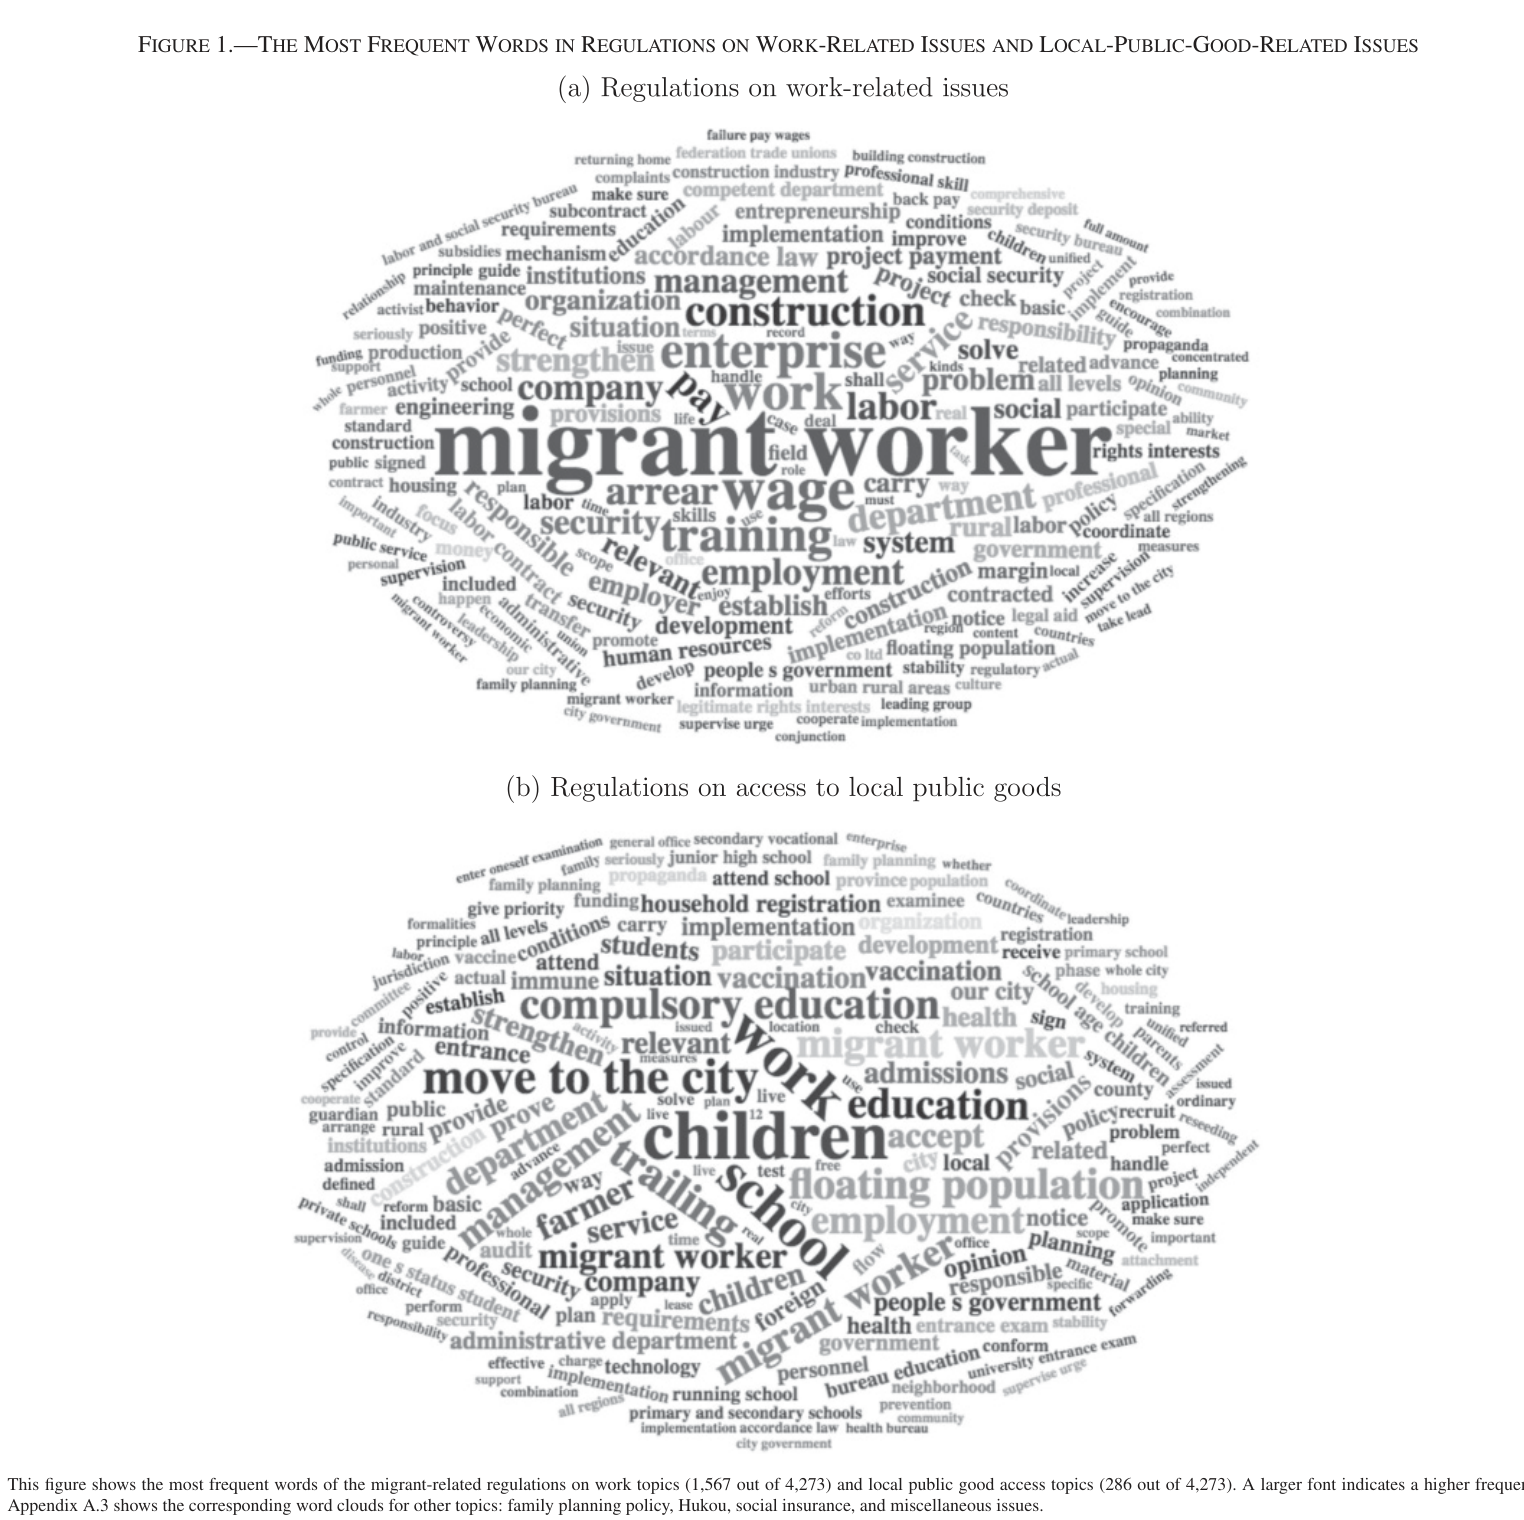
\includegraphics[height=0.62\textheight,width=0.95\textwidth,keepaspectratio]{fig1_wordclouds.png}
    \end{center}
    {\scriptsize\emph{Source: Tian (2024), Figure 1. Original paper figure.}}
\end{frame}

% -----------------------------------------------------------------------------
\begin{frame}{Validation: manual coding and NLP coding tell a similar story}
    \begin{itemize}
        \item Two law-trained research assistants independently coded a subset of regulations.
        \item The author also validates manual coding using three supervised NLP methods:
              \begin{itemize}
                  \item random forest;
                  \item multilayer perceptron;
                  \item convolutional neural network with word embeddings.
              \end{itemize}
        \item Appendix evidence: correlations between NLP scores and manual coding are around 0.71--0.73.
    \end{itemize}

    \vspace{0.4em}
    \begin{center}
        \begin{tabular}{lccc}
            \toprule
            Method                         & RF    & MLP   & CNN   \\
            \midrule
            Correlation with manual coding & 0.734 & 0.728 & 0.712 \\
            \bottomrule
        \end{tabular}
    \end{center}

    \takeaway{The main outcome is text-based, but not purely subjective.}
\end{frame}

% -----------------------------------------------------------------------------
\begin{frame}{Figure 2: a visible break in policy activity after WTO accession}
    \small Reading: before 2001, regulation activity is limited; after 2001, both the number and pro-migrant content of regulations rise sharply.
    \begin{center}
        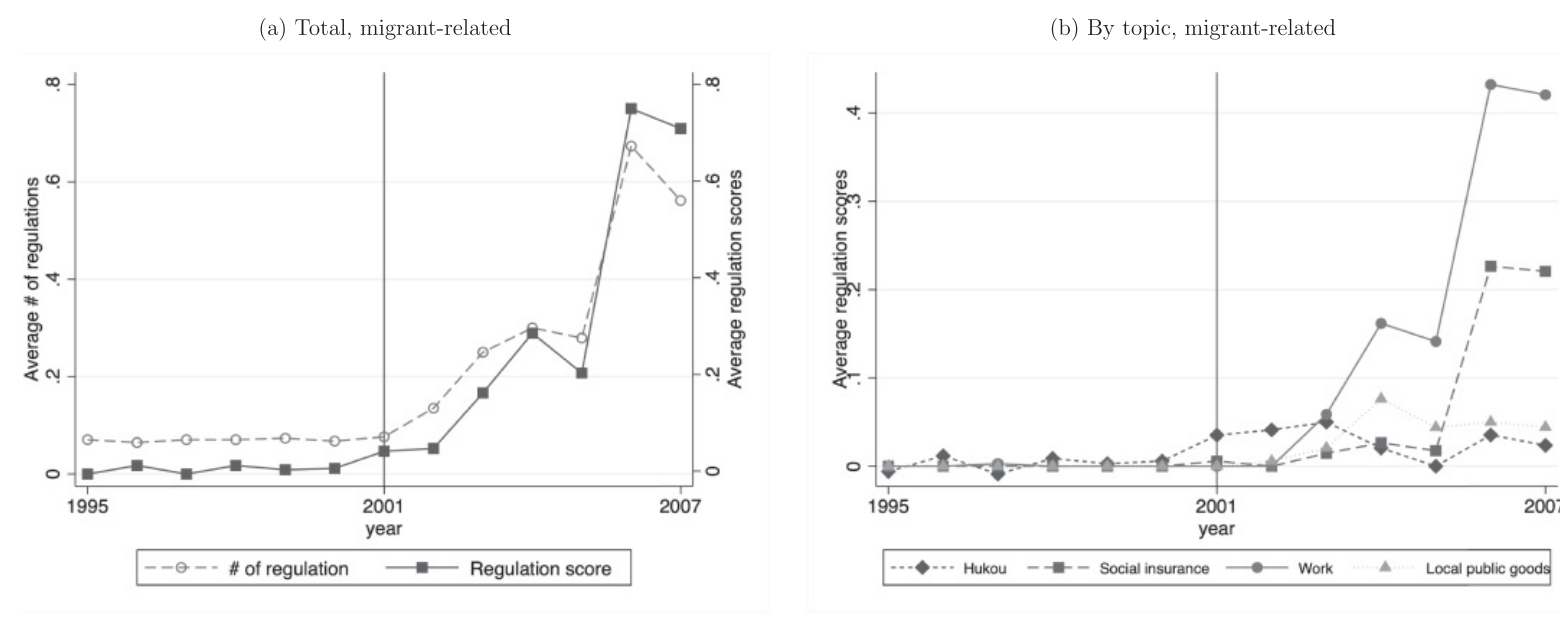
\includegraphics[height=0.62\textheight,width=0.95\textwidth,keepaspectratio]{fig2_panels_ab.png}
    \end{center}
    {\scriptsize\emph{Source: Tian (2024), Figure 2. Original paper figure.}}
\end{frame}

% =============================================================================
\section{Trade Shock and Empirical Design}
% =============================================================================

% -----------------------------------------------------------------------------
\begin{frame}{Measuring exposure to export-market liberalization}
    \begin{itemize}
        \item Industry-level shock: tariff reductions faced by Chinese exporters after WTO accession.
        \item Prefecture exposure is a shift-share measure using pre-WTO industrial employment shares.
    \end{itemize}

    \vspace{0.6em}
    \begin{equation*}
        \Delta \tau_i^{X} = \sum_{s} \omega_{is,2000}\, \Delta \tau_s^{X}
    \end{equation*}

    \begin{itemize}
        \item $\omega_{is,2000}$: prefecture $i$'s 2000 employment share in industry $s$.
        \item $\Delta \tau_s^{X}$: change in foreign tariffs on Chinese exports in industry $s$.
        \item More negative $\Delta \tau_i^{X}$ means greater export-market liberalization.
    \end{itemize}

    \takeaway{Variation is driven by initial industrial composition interacted with externally changing foreign tariffs.}
\end{frame}

% -----------------------------------------------------------------------------
\begin{frame}{Figure 3: export tariffs fell after WTO accession}
    \small Reading: tariff cuts are industry-specific, so prefectures with different initial industrial structures receive different export-market shocks.
    \begin{center}
        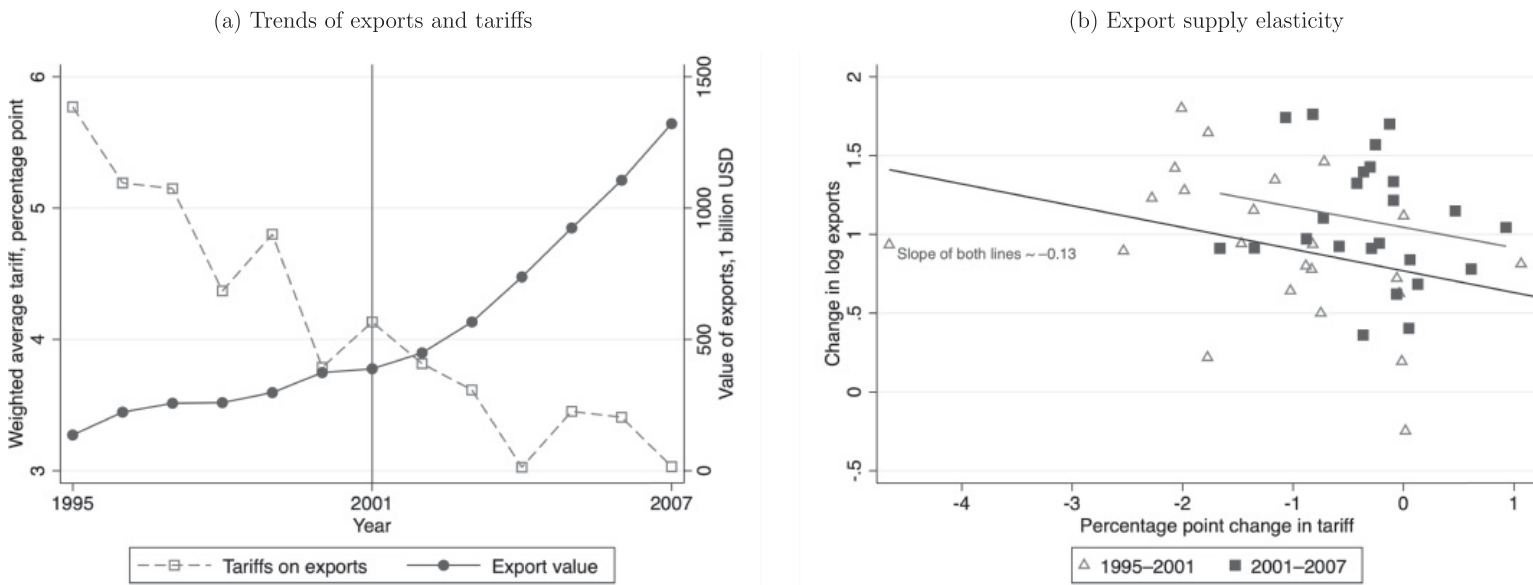
\includegraphics[height=0.62\textheight,width=0.96\textwidth,keepaspectratio]{fig3_tariffs_exports_crop2.png}
    \end{center}
    {\scriptsize\emph{Source: Tian (2024), Figure 3. Original paper figure, cropped to panels.}}
\end{frame}

% -----------------------------------------------------------------------------
\begin{frame}{Long-difference design}
    \begin{itemize}
        \item Main estimating equation:
    \end{itemize}

    \vspace{-0.2em}
    \begin{equation*}
        \Delta R_i^{2001-2007} = \alpha + \beta \Delta \tau_i^{X,2001-2007} + \Gamma X_i + \varepsilon_i,
    \end{equation*}

    \begin{itemize}
        \item $\Delta R_i^{2001-2007}$: change in inverse-hyperbolic-sine regulation score.
        \item $\Delta \tau_i^{X,2001-2007}$: prefecture-level tariff change on exports.
        \item Controls include import tariffs, input tariffs, pre-WTO regulation, PNTR, MFA, and pretrends in some specifications.
    \end{itemize}

    \vspace{0.6em}
    \begin{equation*}
        \beta < 0 \quad \Rightarrow \quad \text{larger tariff cuts lead to more pro-migrant regulation.}
    \end{equation*}

    \takeaway{The identifying comparison is across prefectures, before and after WTO accession.}
\end{frame}

% -----------------------------------------------------------------------------
\begin{frame}{Identification: what must be true?}
    \begin{enumerate}
        \item \textbf{No differential pre-trends.} High-exposure prefectures should not already be on a faster pro-migrant reform path before WTO.
        \item \textbf{Tariff changes are plausibly external.} Foreign tariff cuts should not be chosen because of future Hukou reforms in specific Chinese prefectures.
        \item \textbf{Initial industrial shares are not merely proxying for local governance quality.} Export-oriented cities may also differ in marketization, fiscal capacity, and policy responsiveness.
        \item \textbf{Other WTO channels are controlled.} Import competition, input tariffs, PNTR uncertainty, and MFA quota removal may confound the export-demand interpretation.
    \end{enumerate}

    \takeaway{The paper's credibility rests on pre-trend tests and robustness to alternative WTO-related shocks and controls.}
\end{frame}

% -----------------------------------------------------------------------------
\begin{frame}{Figure 4A: industry-level pre-trends}
    \small Reading: post-WTO tariff reductions are not strongly predicted by pre-WTO export growth or tariff trends at the industry level.
    \begin{center}
        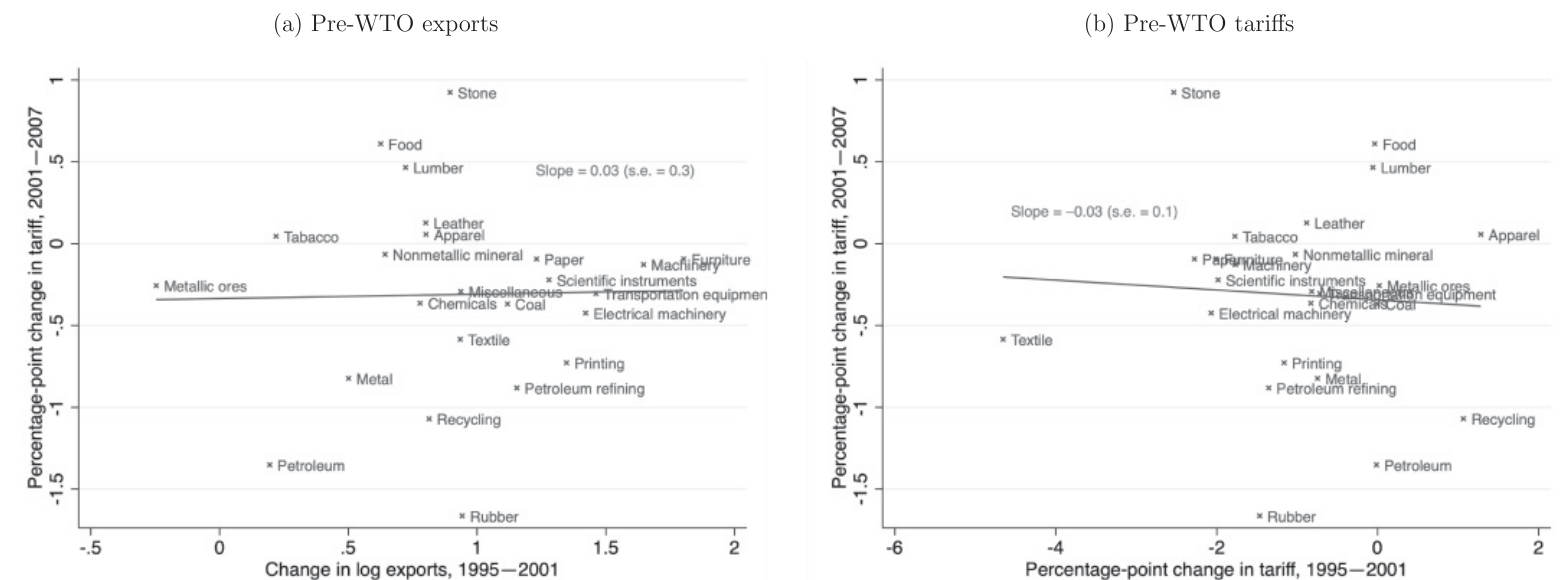
\includegraphics[height=0.62\textheight,width=0.96\textwidth,keepaspectratio]{fig4_industry_pretrends_crop2.png}
    \end{center}
    {\scriptsize\emph{Source: Tian (2024), Figure 4. Original paper figure, cropped to panels.}}
\end{frame}

% -----------------------------------------------------------------------------
\begin{frame}{Figure 4B: prefecture-level pre-trends}
    \small Reading: regions more exposed after 2001 do not look systematically more reformist before 2001.
    \begin{center}
        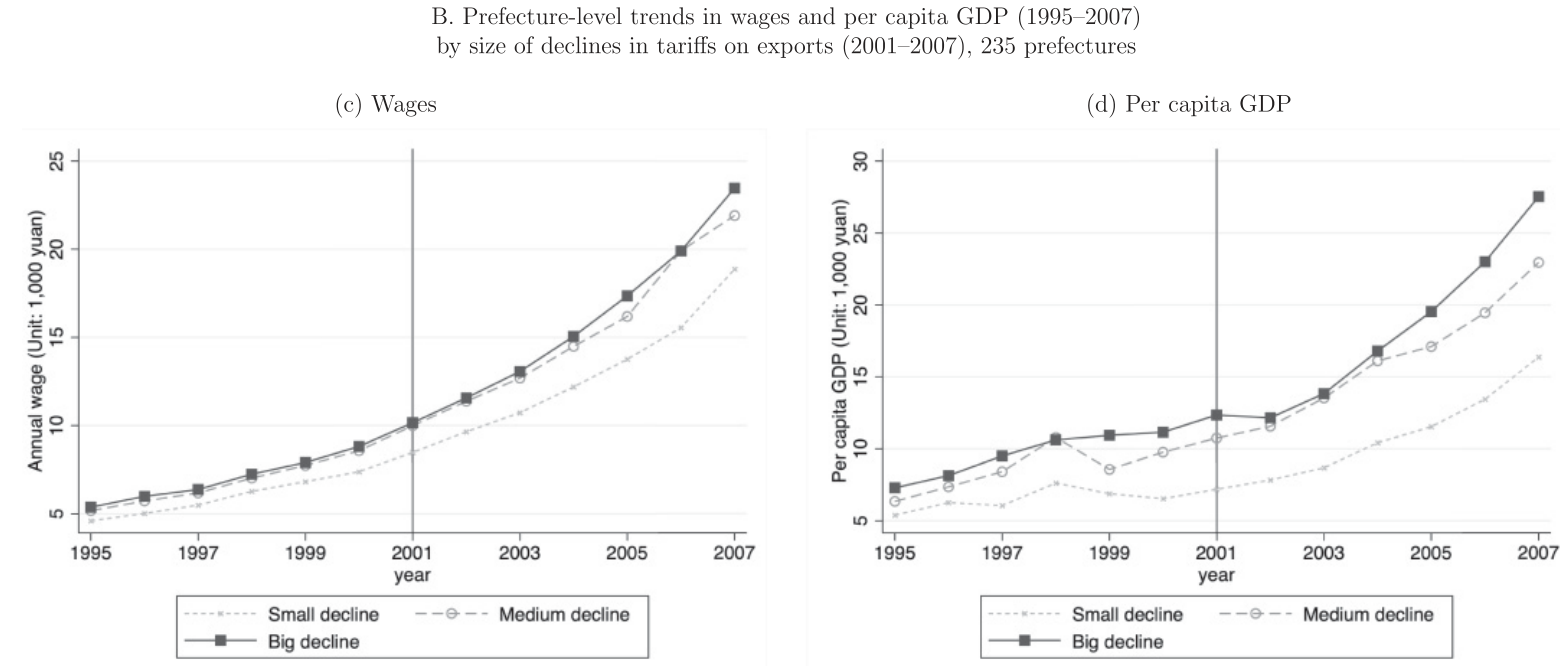
\includegraphics[height=0.62\textheight,width=0.96\textwidth,keepaspectratio]{fig4_prefecture_pretrends_crop2.png}
    \end{center}
    {\scriptsize\emph{Source: Tian (2024), Figure 4. Original paper figure, cropped to panels.}}
\end{frame}

% =============================================================================
\section{Main Results}
% =============================================================================

% -----------------------------------------------------------------------------
\begin{frame}{Table 1: export-market liberalization predicts pro-migrant reform}
    \small
    \begin{center}
        \begin{tabular}{lcccc}
            \toprule
            Dependent variable: $\Delta\sinhinv(\text{regulation score})$ & (1)           & (3)           & (5)           & (7)         \\
            \midrule
            $\Delta$ tariffs on exports, 2001--2007                       & $-1.04^{***}$ & $-1.48^{***}$ & $-1.60^{***}$ & $-1.02^{*}$ \\
                                                                          & $(0.30)$      & $(0.33)$      & $(0.50)$      & $(0.53)$    \\
            $\Delta$ tariffs on imports                                   & $-0.03$       & $-0.05$       & $-0.11^{**}$  & $-0.08$     \\
            $\Delta$ tariffs on inputs                                    & $-0.54^{***}$ & $-0.53^{***}$ & $-0.31^{**}$  & $-0.13$     \\
            Controls for other WTO shocks                                 & No            & No            & Yes           & Yes         \\
            Additional pre-trend controls                                 & No            & No            & No            & Yes         \\
            Observations                                                  & 333           & 317           & 248           & 235         \\
            R-squared                                                     & 0.09          & 0.11          & 0.08          & 0.15        \\
            \bottomrule
        \end{tabular}
    \end{center}
    \vspace{0.2em}
    \scriptsize Notes: selected columns from Tian (2024), Table 1, Panel A. Standard errors in parentheses in the paper. $^{*}p<0.1$, $^{**}p<0.05$, $^{***}p<0.01$.

    \takeaway{The coefficient is consistently negative: because tariff changes are negative cuts, the result means larger export liberalization raises migrant-friendliness.}
\end{frame}

% -----------------------------------------------------------------------------
\begin{frame}{Figure 5: reduced-form relationship in the data}
    \small Reading: more negative export-tariff changes are associated with larger increases in pro-migrant regulation.
    \begin{center}
        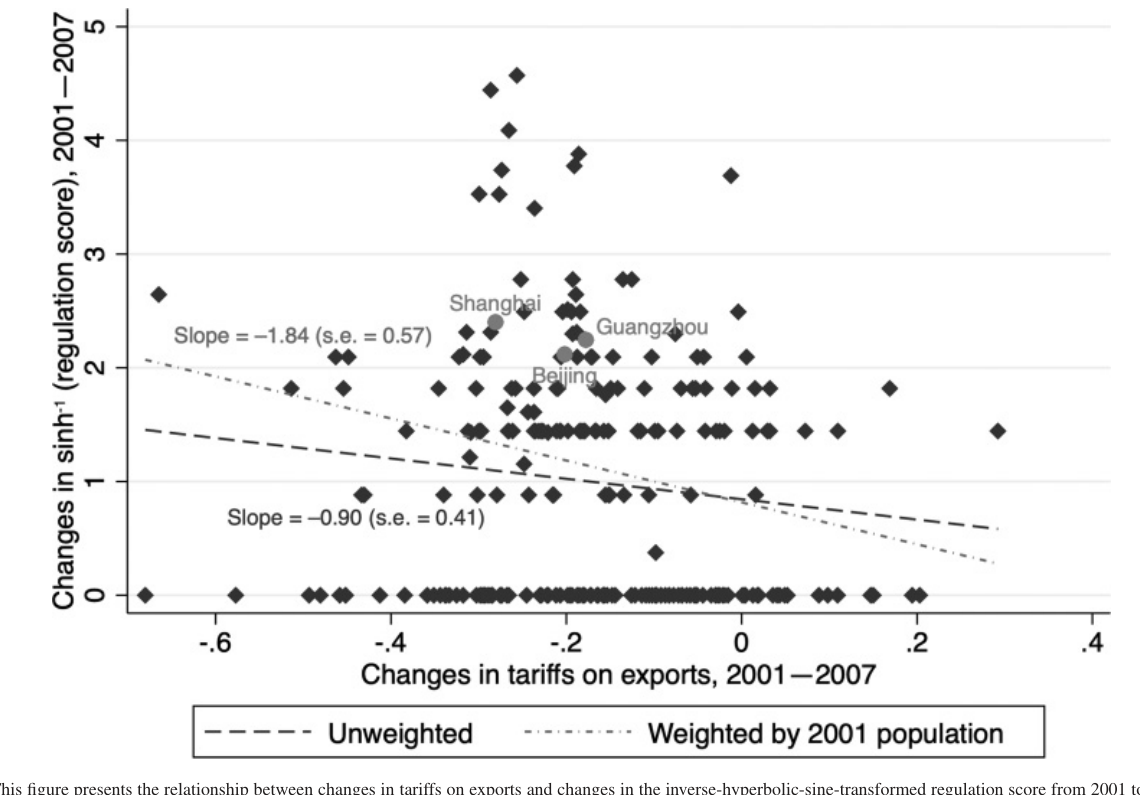
\includegraphics[height=0.62\textheight,width=0.96\textwidth,keepaspectratio]{fig5_main_scatter_crop2.png}
    \end{center}
    {\scriptsize\emph{Source: Tian (2024), Figure 5. Original paper figure, cropped to panel.}}
\end{frame}

% -----------------------------------------------------------------------------
\begin{frame}{How large is the effect?}
    \begin{itemize}
        \item The paper reports that prefectures in the upper third of export-market liberalization increased regulation scores by about 0.40 standard deviations more than prefectures in the lower third.
        \item This is an economically meaningful institutional response over only six years.
        \item Interpretation should remain precise: the result is about formal local regulations, not necessarily full equalization of urban citizenship.
    \end{itemize}

    \vspace{0.6em}
    \begin{equation*}
        \text{Trade shock} \rightarrow \text{de jure pro-migrant reform} \neq \text{complete Hukou abolition.}
    \end{equation*}

    \takeaway{The paper identifies a margin of institutional adaptation, not the end of the Hukou system.}
\end{frame}

% -----------------------------------------------------------------------------
\begin{frame}{Robustness: the result is not driven by a single coding or specification}
    \begin{itemize}
        \item Alternative regulation scores: manual coding and random-forest coding produce similar results.
        \item Alternative export shocks: PNTR and MFA quota reductions generate similar reform responses.
        \item Alternative specifications: panel specifications, score levels, alternative Bartik exposure, and industrial-composition controls.
        \item Inference: bootstrap and AKM p-values are reported for shift-share concerns.
    \end{itemize}

    \vspace{0.4em}
    \begin{center}
        \begin{tabular}{lcc}
            \toprule
            Outcome coding & Core export-tariff coefficient range & Interpretation                              \\
            \midrule
            Manual coding  & $-0.91$ to $-1.60$                   & Larger tariff cuts, more pro-migrant reform \\
            Random forest  & $-0.86$ to $-1.46$                   & Similar sign and magnitude                  \\
            \bottomrule
        \end{tabular}
    \end{center}

    \takeaway{The evidence is not a single fragile coefficient, although the identification still relies on the shift-share design.}
\end{frame}

% -----------------------------------------------------------------------------
\begin{frame}{Table 2: heterogeneity supports the labor-demand mechanism}
    \small
    \begin{center}
        \begin{tabular}{lcccc}
            \toprule
            Baseline characteristic                                     & Migrant intensity & Private firm share & Log GDP p.c. & Log wage     \\
            \midrule
            Interaction: $\Delta$ export tariff $\times$ characteristic & $-21.89^{*}$      & $-6.14^{***}$      & $-1.47^{**}$ & $-4.18^{**}$ \\
                                                                        & $(11.46)$         & $(1.20)$           & $(0.66)$     & $(2.01)$     \\
            Additional controls                                         & Yes               & Yes                & Yes          & Yes          \\
            Observations                                                & 235               & 235                & 235          & 235          \\
            R-squared                                                   & 0.16              & 0.20               & 0.27         & 0.21         \\
            \bottomrule
        \end{tabular}
    \end{center}
    \vspace{0.2em}
    \scriptsize Notes: selected columns from Tian (2024), Table 2. Dependent variable: change in $\sinhinv$(regulation score), manual coding, 2001--2007.

    \takeaway{High migrant intensity, private-sector presence, and richer labor markets strengthen the reform response, consistent with labor-demand incentives.}
\end{frame}

% -----------------------------------------------------------------------------
\begin{frame}{Figure 6: visualizing heterogeneity}
    \small Reading: the effect is stronger where migrants are more economically relevant to local growth and private-sector production.
    \begin{center}
        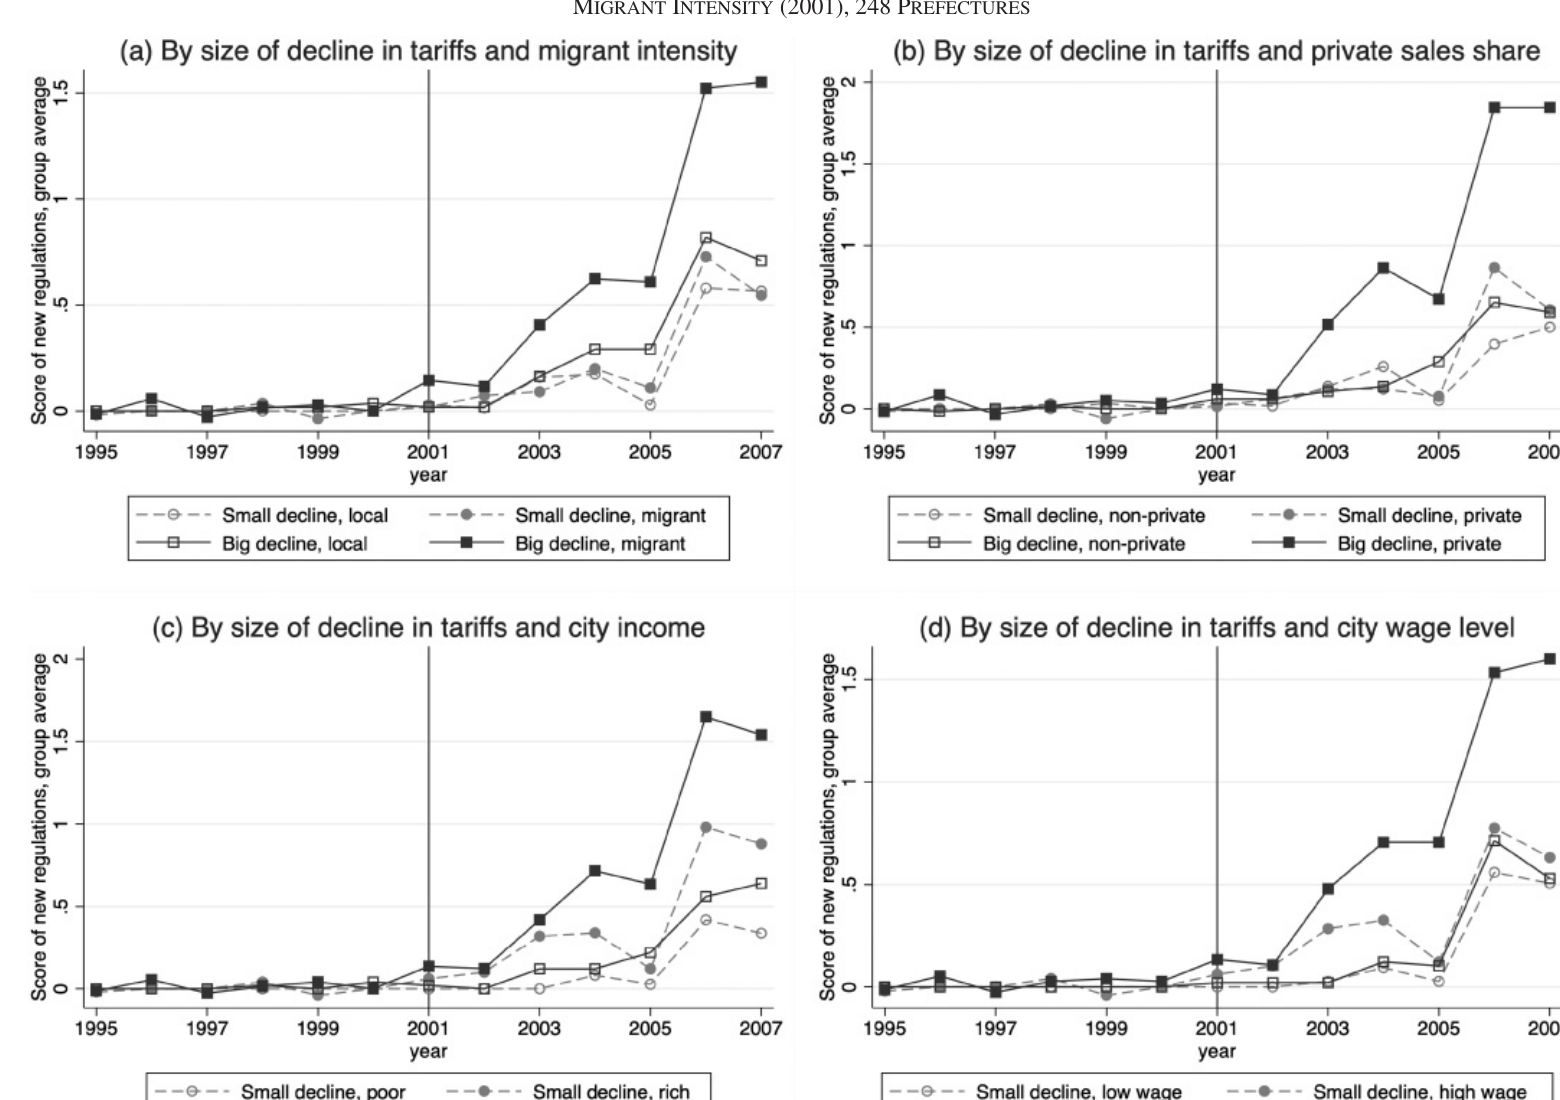
\includegraphics[height=0.62\textheight,width=0.96\textwidth,keepaspectratio]{fig6_heterogeneity_crop2.png}
    \end{center}
    {\scriptsize\emph{Source: Tian (2024), Figure 6. Original paper figure, cropped to panels.}}
\end{frame}

% =============================================================================
\section{Interpretation: Welfare and Migration Flows}
% =============================================================================

% -----------------------------------------------------------------------------
\begin{frame}{Table 3: do pro-migrant regulations correspond to better migrant outcomes?}
    \scriptsize
    \begin{center}
        \begin{tabular}{lccccc}
            \toprule
            Migrant outcome in 2005            & Unemp. ins. & Pension     & Medical ins. & Contract months & Monthly income \\
            \midrule
            $\sinhinv$(regulation score), 2005 & $0.01^{*}$  & $0.02^{**}$ & $0.02^{**}$  & $0.09$          & $29.27^{**}$   \\
                                               & $(0.01)$    & $(0.01)$    & $(0.01)$     & $(0.10)$        & $(13.98)$      \\
            Local outcome control              & Yes         & Yes         & Yes          & Yes             & Yes            \\
            Observations                       & 246         & 246         & 246          & 246             & 246            \\
            \bottomrule
        \end{tabular}
    \end{center}
    \vspace{0.3em}
    \small
    The table is not the main causal design; it is a validation exercise showing that places with higher migrant-friendliness also have better observed migrant welfare in 2005.

    \takeaway{The regulation score appears to capture meaningful de facto migrant conditions, but enforcement is only indirectly measured.}
\end{frame}

% -----------------------------------------------------------------------------
\begin{frame}{Table 4: trade shocks, regulation changes, and migrant flows}
    \scriptsize
    \begin{center}
        \begin{tabular}{lcccc}
            \toprule
            Dependent variable                 & Migrant share & Short-distance migrants & Medium-distance migrants & Long-distance migrants \\
            \midrule
            $\Delta$ tariffs on exports        & $-6.23^{*}$   & $-1.18^{***}$           & $-0.39^{**}$             & $0.16$                 \\
                                               & $(3.22)$      & $(0.27)$                & $(0.17)$                 & $(0.39)$               \\
            $\Delta\sinhinv$(regulation score) & $0.87^{***}$  & $0.20^{***}$            & $0.05^{*}$               & $0.08^{*}$             \\
                                               & $(0.22)$      & $(0.04)$                & $(0.03)$                 & $(0.04)$               \\
            Observations                       & 248           & 238                     & 248                      & 247                    \\
            \bottomrule
        \end{tabular}
    \end{center}
    \vspace{0.3em}
    \small
    The migration-flow evidence is consistent with the mechanism, but it is harder to interpret causally because trade can attract migrants directly through wages and jobs.

    \takeaway{The strongest causal claim remains trade exposure causing regulation changes; the migration-flow channel is supporting evidence.}
\end{frame}

% -----------------------------------------------------------------------------
\begin{frame}{What this paper teaches about China's WTO accession}
    \begin{itemize}
        \item WTO accession did not only change exports, prices, and firm behavior.
        \item It also changed the local political economy of labor-market governance.
        \item Local governments facing larger export opportunities had stronger incentives to reduce mobility frictions.
        \item The paper therefore adds an institutional channel to the China-WTO literature.
    \end{itemize}

    \vspace{0.8em}
    \begin{equation*}
        \text{External liberalization} \quad \Rightarrow \quad \text{domestic institutional adaptation.}
    \end{equation*}

    \takeaway{The contribution is strongest when framed as trade-induced institutional adaptation, not as a general theory of Hukou reform.}
\end{frame}

% =============================================================================
\section{Critical Assessment}
% =============================================================================

% -----------------------------------------------------------------------------
\begin{frame}{Critique from Hukou political and historical scholarship}
    \begin{itemize}
        \item \textbf{Hukou is more than a labor-market friction.} Historical and political studies stress social control, state capacity, rural-urban hierarchy, fiscal citizenship, and public-security governance.
        \item \textbf{Functional reform is not equal citizenship.} Pro-migrant policies may help retain workers while preserving exclusion from full urban welfare rights.
        \item \textbf{Local discretion is politically bounded.} Prefecture reforms occur within central constraints; the paper's local-government optimization story may understate vertical political authority.
        \item \textbf{Textual reform may institutionalize selective inclusion.} New rules can formalize partial access rather than dismantle the underlying classification system.
    \end{itemize}

    \takeaway{The paper's economic mechanism is convincing, but it should be read as a theory of marginal policy adjustment within a durable political institution.}
\end{frame}

% -----------------------------------------------------------------------------
\begin{frame}{Critique of the empirical design}
    \begin{enumerate}
        \item \textbf{Shift-share concern.} Initial industrial composition may proxy for marketization, coastal openness, administrative capacity, or export-oriented governance.
        \item \textbf{Policy timing concern.} Post-2001 local reforms may also reflect national labor-law modernization and urban governance campaigns.
        \item \textbf{Outcome measurement.} Regulation texts are observable, but enforcement intensity is not directly measured.
        \item \textbf{Mechanism separation.} Trade liberalization may affect migration directly through wages and jobs, indirectly through regulations, or through fiscal capacity.
        \item \textbf{Welfare interpretation.} The paper documents reform responses, but does not quantify general-equilibrium welfare gains or distributional costs.
    \end{enumerate}

    \takeaway{The reduced form is strong; the exact channel and welfare meaning are less fully pinned down.}
\end{frame}

% -----------------------------------------------------------------------------
\begin{frame}{How we briefing this paper}
    \begin{itemize}
        \item \textbf{What the paper establishes well:} WTO-induced export-market liberalization caused more pro-migrant regulation at the prefecture level.
        \item \textbf{What it suggests:} migration-policy changes were economically meaningful and related to migrant welfare and flows.
        \item \textbf{What it does not fully prove:} regulation enforcement, causal mediation through migrant flows, and welfare effects.
        \item \textbf{Why it matters:} it shows that globalization can change not only market outcomes but also domestic institutions that govern factor mobility.
    \end{itemize}

    \vspace{0.6em}
    \begin{equation*}
        \text{Trade openness changes incentives; incentives reshape institutions at the margin.}
    \end{equation*}
\end{frame}

% -----------------------------------------------------------------------------
\begin{frame}[plain]
    \centering
    \vspace{2.5cm}
    {\Large Questions and discussion}
\end{frame}

% =============================================================================
\appendix
\section{Backup: Original Tables}
% =============================================================================

\begin{frame}{Backup: full Table 1 from the paper}
    \begin{center}
        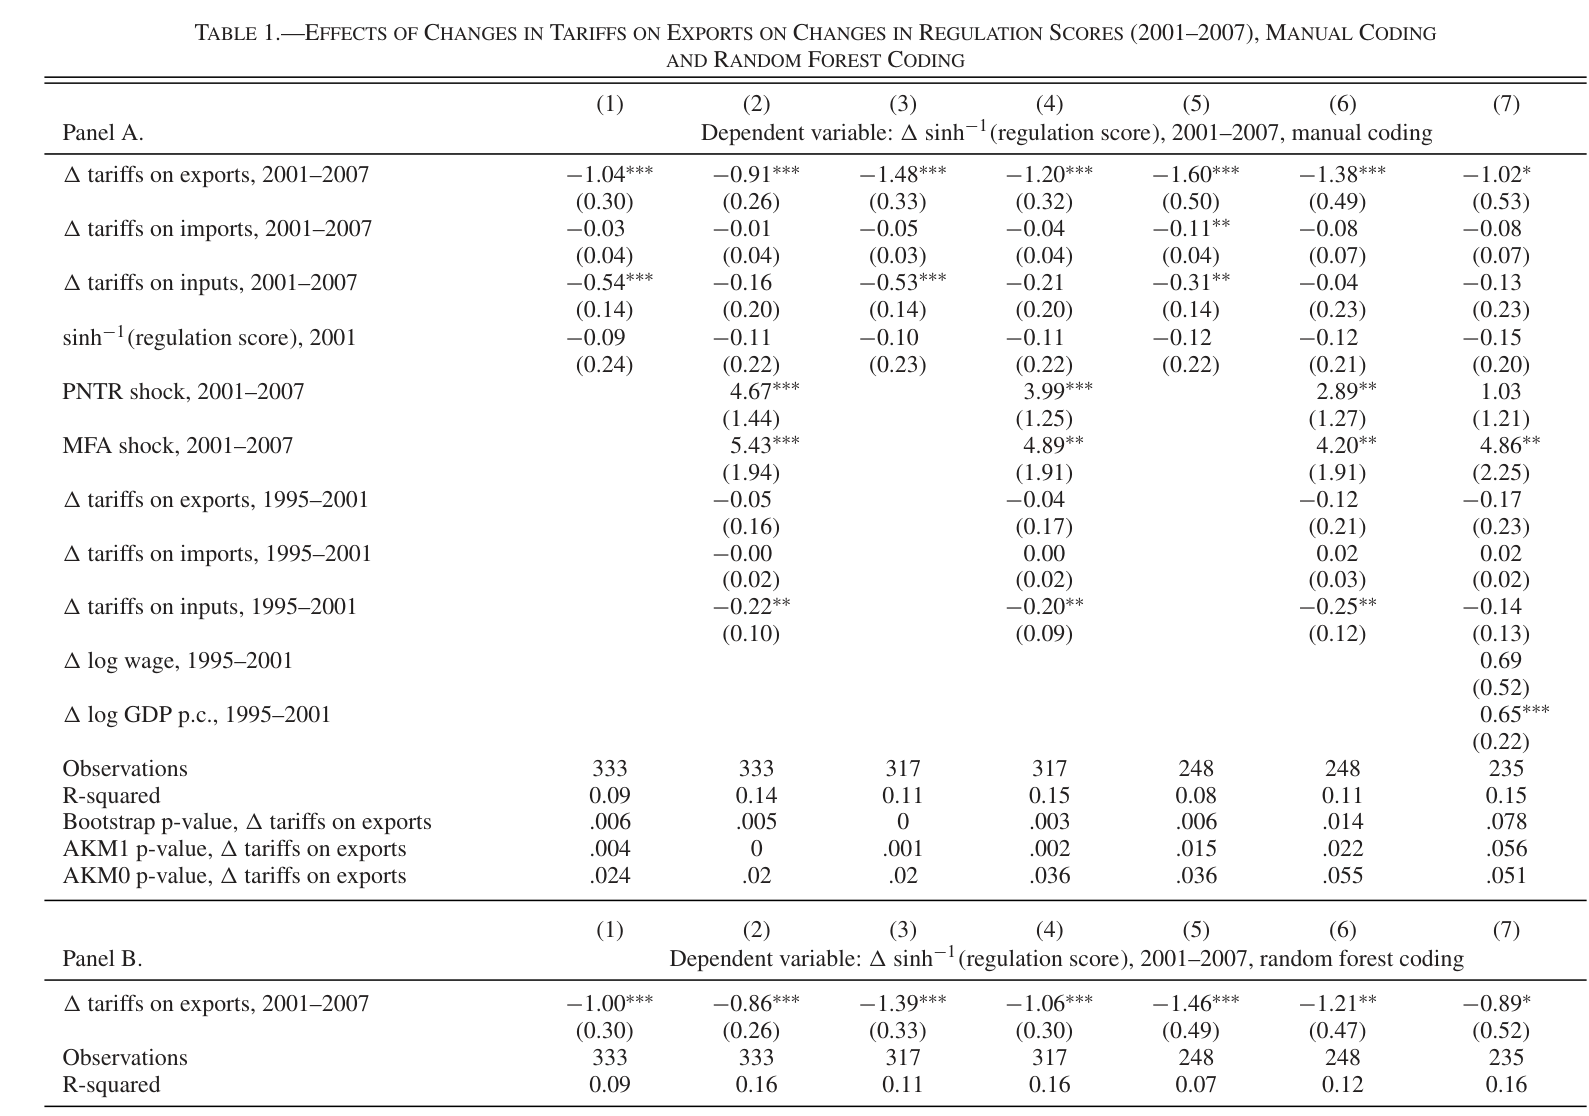
\includegraphics[width=0.97\textwidth,height=0.78\textheight,keepaspectratio]{table1_main_results.png}
    \end{center}
\end{frame}

\begin{frame}{Backup: full Table 2 from the paper}
    \begin{center}
        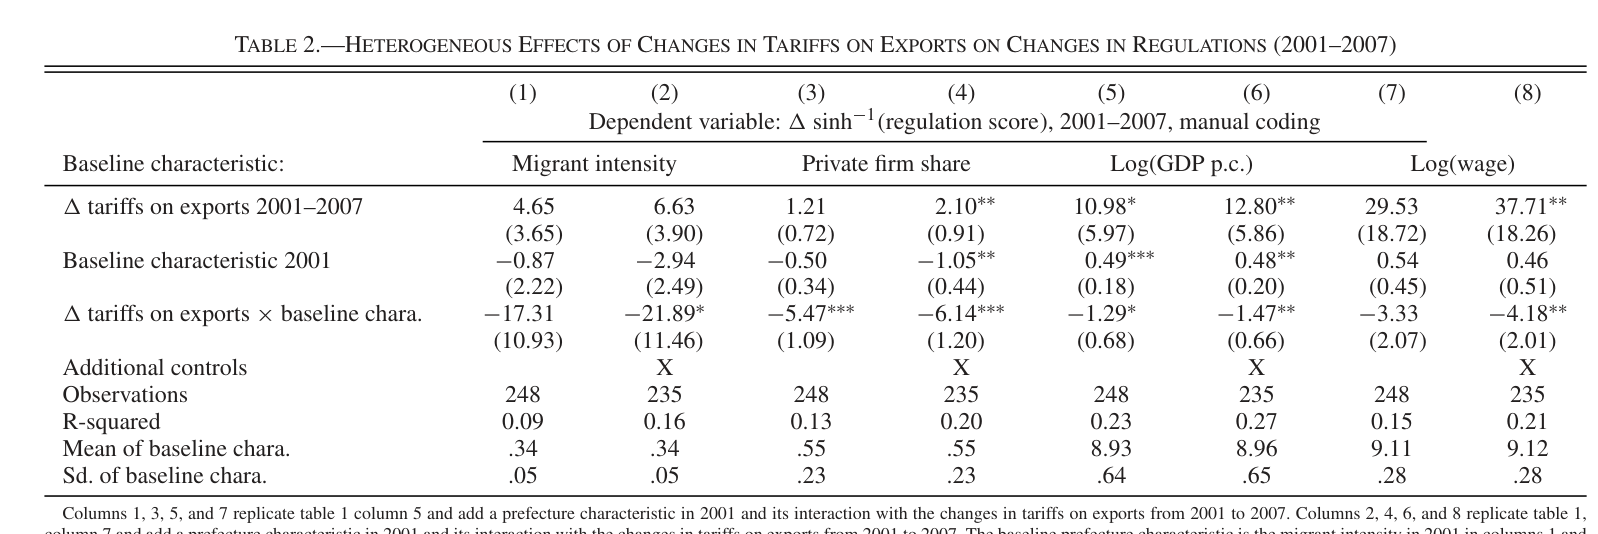
\includegraphics[width=0.97\textwidth,height=0.78\textheight,keepaspectratio]{table2_heterogeneity.png}
    \end{center}
\end{frame}

\begin{frame}{Backup: full Table 3 from the paper}
    \begin{center}
        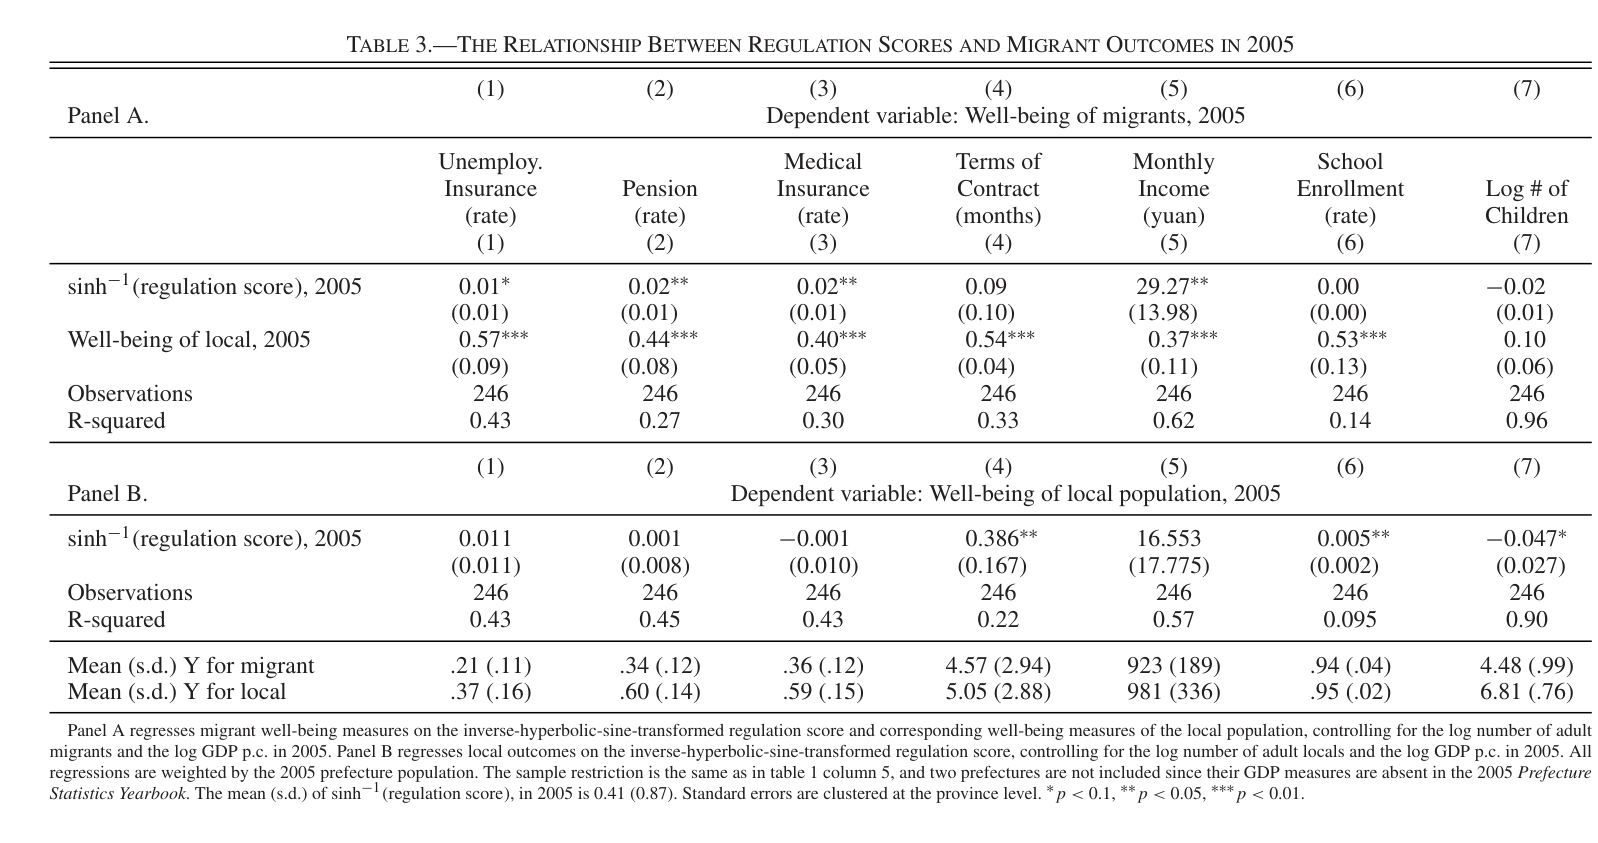
\includegraphics[width=0.97\textwidth,height=0.78\textheight,keepaspectratio]{table3_wellbeing.png}
    \end{center}
\end{frame}

\begin{frame}{Backup: full Table 4 from the paper}
    \begin{center}
        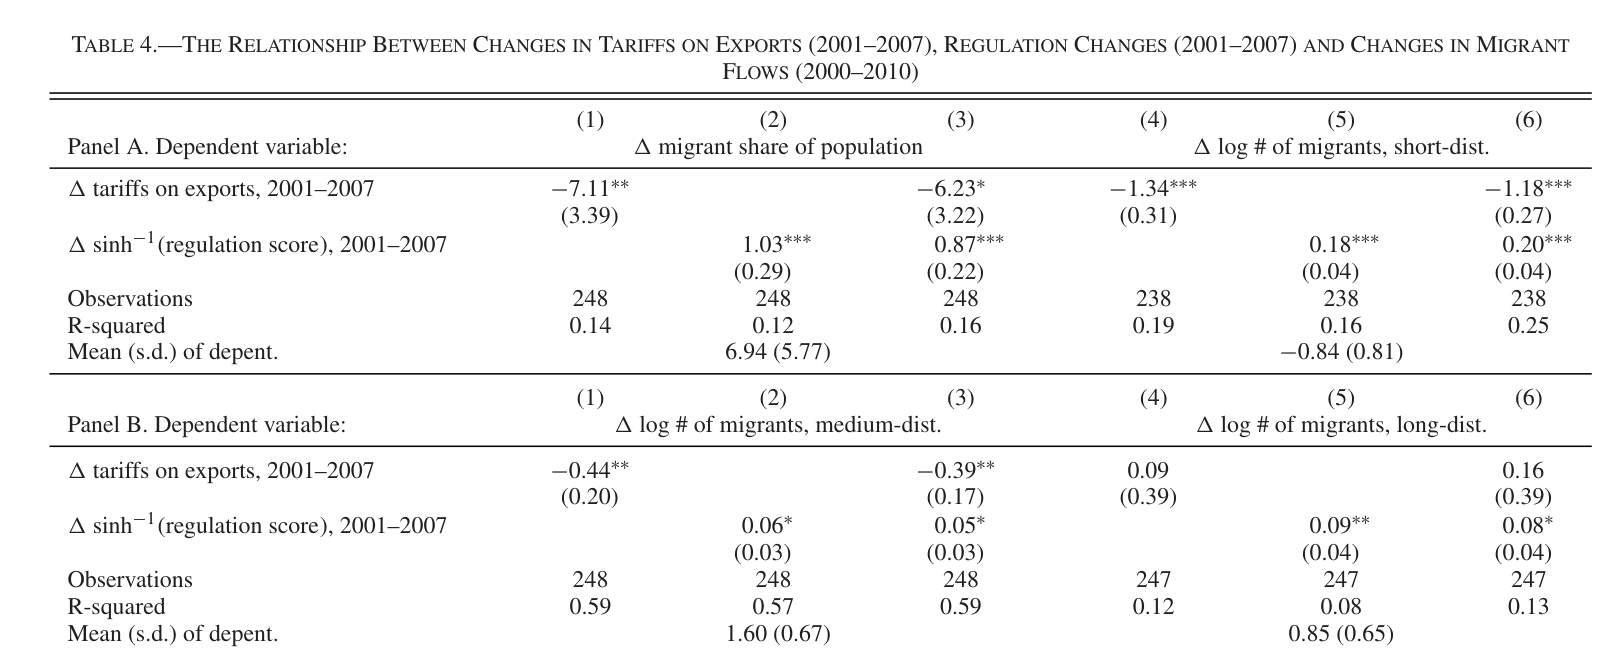
\includegraphics[width=0.97\textwidth,height=0.78\textheight,keepaspectratio]{table4_migration_flows.png}
    \end{center}
\end{frame}

\end{document}
